% Options for packages loaded elsewhere
\PassOptionsToPackage{unicode}{hyperref}
\PassOptionsToPackage{hyphens}{url}
\documentclass[
]{article}
\usepackage{xcolor}
\usepackage{amsmath,amssymb}
\setcounter{secnumdepth}{-\maxdimen} % remove section numbering
\usepackage{iftex}
\ifPDFTeX
  \usepackage[T1]{fontenc}
  \usepackage[utf8]{inputenc}
  \usepackage{textcomp} % provide euro and other symbols
\else % if luatex or xetex
  \usepackage{unicode-math} % this also loads fontspec
  \defaultfontfeatures{Scale=MatchLowercase}
  \defaultfontfeatures[\rmfamily]{Ligatures=TeX,Scale=1}
\fi
\usepackage{lmodern}
\ifPDFTeX\else
  % xetex/luatex font selection
\fi
% Use upquote if available, for straight quotes in verbatim environments
\IfFileExists{upquote.sty}{\usepackage{upquote}}{}
\IfFileExists{microtype.sty}{% use microtype if available
  \usepackage[]{microtype}
  \UseMicrotypeSet[protrusion]{basicmath} % disable protrusion for tt fonts
}{}
\makeatletter
\@ifundefined{KOMAClassName}{% if non-KOMA class
  \IfFileExists{parskip.sty}{%
    \usepackage{parskip}
  }{% else
    \setlength{\parindent}{0pt}
    \setlength{\parskip}{6pt plus 2pt minus 1pt}}
}{% if KOMA class
  \KOMAoptions{parskip=half}}
\makeatother
\usepackage{graphicx}
\makeatletter
\newsavebox\pandoc@box
\newcommand*\pandocbounded[1]{% scales image to fit in text height/width
  \sbox\pandoc@box{#1}%
  \Gscale@div\@tempa{\textheight}{\dimexpr\ht\pandoc@box+\dp\pandoc@box\relax}%
  \Gscale@div\@tempb{\linewidth}{\wd\pandoc@box}%
  \ifdim\@tempb\p@<\@tempa\p@\let\@tempa\@tempb\fi% select the smaller of both
  \ifdim\@tempa\p@<\p@\scalebox{\@tempa}{\usebox\pandoc@box}%
  \else\usebox{\pandoc@box}%
  \fi%
}
% Set default figure placement to htbp
\def\fps@figure{htbp}
\makeatother
\setlength{\emergencystretch}{3em} % prevent overfull lines
\providecommand{\tightlist}{%
  \setlength{\itemsep}{0pt}\setlength{\parskip}{0pt}}
\usepackage{bookmark}
\IfFileExists{xurl.sty}{\usepackage{xurl}}{} % add URL line breaks if available
\urlstyle{same}
\hypersetup{
  pdftitle={09.10.24 (Лекция)},
  hidelinks,
  pdfcreator={LaTeX via pandoc}}

\title{09.10.24 (Лекция)}
\author{}
\date{}

\begin{document}
\maketitle

\section{Тема: Решение СЛАУ методом QR разложения (метод отражений, или
метод
Хаусхофера)}\label{ux442ux435ux43cux430-ux440ux435ux448ux435ux43dux438ux435-ux441ux43bux430ux443-ux43cux435ux442ux43eux434ux43eux43c-qr-ux440ux430ux437ux43bux43eux436ux435ux43dux438ux44f-ux43cux435ux442ux43eux434-ux43eux442ux440ux430ux436ux435ux43dux438ux439-ux438ux43bux438-ux43cux435ux442ux43eux434-ux445ux430ux443ux441ux445ux43eux444ux435ux440ux430}

\subsection{\texorpdfstring{1. {}
разложение}{1.  разложение}}\label{ux440ux430ux437ux43bux43eux436ux435ux43dux438ux435}

{}\strut \\
{}- ортогональная матрица ({})\\
{}

\begin{enumerate}
\tightlist
\item
  {}
\item
  {} - система матр\\
  {} существует для любой матрицы А\\
  {}\strut \\
  Разложение не единственно\\
  Мы же рассмотрим только один метод для расчета этого разложения
\end{enumerate}

\subsection{2. Матрица отражения
(Хаусхолдера)}\label{ux43cux430ux442ux440ux438ux446ux430-ux43eux442ux440ux430ux436ux435ux43dux438ux44f-ux445ux430ux443ux441ux445ux43eux43bux434ux435ux440ux430}

Представим, что у нас в некотором пространстве есть пространство и
вектор, который нужно отразить относительно него\\

\pandocbounded{\includegraphics[keepaspectratio]{blob:app://obsidian.md/b4f823a8-8206-4e94-b74a-5916b81a3495}}

\hfill\break
{}\\
{}\strut \\
{}\strut \\
{}- матрица отражений

\subsubsection{Основные свойства матрицы
отражений:}\label{ux43eux441ux43dux43eux432ux43dux44bux435-ux441ux432ux43eux439ux441ux442ux432ux430-ux43cux430ux442ux440ux438ux446ux44b-ux43eux442ux440ux430ux436ux435ux43dux438ux439}

\paragraph{\texorpdfstring{1. {} - ортогональная
матрица:}{1.  - ортогональная матрица:}}\label{ux43eux440ux442ux43eux433ux43eux43dux430ux43bux44cux43dux430ux44f-ux43cux430ux442ux440ux438ux446ux430}

{}\strut \\
{}

\paragraph{\texorpdfstring{2. Матрица {}
симметричная:}{2. Матрица  симметричная:}}\label{ux43cux430ux442ux440ux438ux446ux430-ux441ux438ux43cux43cux435ux442ux440ux438ux447ux43dux430ux44f}

{} по определению

\paragraph{3. Матрица инверсивна (сама себе
обратна):}\label{ux43cux430ux442ux440ux438ux446ux430-ux438ux43dux432ux435ux440ux441ux438ux432ux43dux430-ux441ux430ux43cux430-ux441ux435ux431ux435-ux43eux431ux440ux430ux442ux43dux430}

{} из пункта 2

\paragraph{\texorpdfstring{4. Матрица отражений {} имеет {} собственных
значений, равных {}, и одно, равное
{}}{4. Матрица отражений  имеет  собственных значений, равных , и одно, равное }}\label{ux43cux430ux442ux440ux438ux446ux430-ux43eux442ux440ux430ux436ux435ux43dux438ux439-ux438ux43cux435ux435ux442-ux441ux43eux431ux441ux442ux432ux435ux43dux43dux44bux445-ux437ux43dux430ux447ux435ux43dux438ux439-ux440ux430ux432ux43dux44bux445-ux438-ux43eux434ux43dux43e-ux440ux430ux432ux43dux43eux435}

{}\strut \\
{}-собственное значение\\
{}\strut \\
{} - собственный вектор\\
{} - собственный вектор\\
\#Бля я тут не понял нифига

\paragraph{\texorpdfstring{5. {} - не является собственно
ортогональной}{5.  - не является собственно ортогональной}}\label{ux43dux435-ux44fux432ux43bux44fux435ux442ux441ux44f-ux441ux43eux431ux441ux442ux432ux435ux43dux43dux43e-ux43eux440ux442ux43eux433ux43eux43dux430ux43bux44cux43dux43eux439}

{}

\subsubsection{Рациональный способ разложения -Умножение матриц
Хаусхофера}\label{ux440ux430ux446ux438ux43eux43dux430ux43bux44cux43dux44bux439-ux441ux43fux43eux441ux43eux431-ux440ux430ux437ux43bux43eux436ux435ux43dux438ux44f--ux443ux43cux43dux43eux436ux435ux43dux438ux435-ux43cux430ux442ux440ux438ux446-ux445ux430ux443ux441ux445ux43eux444ux435ux440ux430}

\begin{verbatim}
$Ha=(I-\frac{2\overline{u}\overline{u}^T}{\overline{u}^T\overline{u}})a=a-\frac{2\overline{u}\overline{u}^{T}{a}}{\overline{u}^T\overline{u}}=a-\lambda{u}$
$K=\frac{u^{T}u}{2};\ \lambda=\frac{u^{T}a}{K}$
Копировать
\end{verbatim}

\subsubsection{Задача об обнулении
подвектора:}\label{ux437ux430ux434ux430ux447ux430-ux43eux431-ux43eux431ux43dux443ux43bux435ux43dux438ux438-ux43fux43eux434ux432ux435ux43aux442ux43eux440ux430}

{}\strut \\
{}\strut \\
где {} и {}

\paragraph{Доказательство:}\label{ux434ux43eux43aux430ux437ux430ux442ux435ux43bux44cux441ux442ux432ux43e}

{}\strut \\
{}\strut \\
{}\strut \\
{}

\paragraph{Пример:}\label{ux43fux440ux438ux43cux435ux440}

Занулим этот вектор:\\
{}Все дальше делалось на компе {[}сорян{]}

\subsubsection{4. Решение СЛАУ методом отражений и построение QR
разложения
матрицы}\label{ux440ux435ux448ux435ux43dux438ux435-ux441ux43bux430ux443-ux43cux435ux442ux43eux434ux43eux43c-ux43eux442ux440ux430ux436ux435ux43dux438ux439-ux438-ux43fux43eux441ux442ux440ux43eux435ux43dux438ux435-qr-ux440ux430ux437ux43bux43eux436ux435ux43dux438ux44f-ux43cux430ux442ux440ux438ux446ux44b}

\begin{enumerate}
\tightlist
\item
  Подбираем матрицу {} так, чтобы поддиагональные элементы матрицы {}
  обнулялись:\\

  \pandocbounded{\includegraphics[keepaspectratio]{blob:app://obsidian.md/a0b40335-7626-4bce-ba86-d1f5d912d2fe}}

  \hfill\break
  \#Бля вот фото лучше, позже перепиши\\
  \pandocbounded{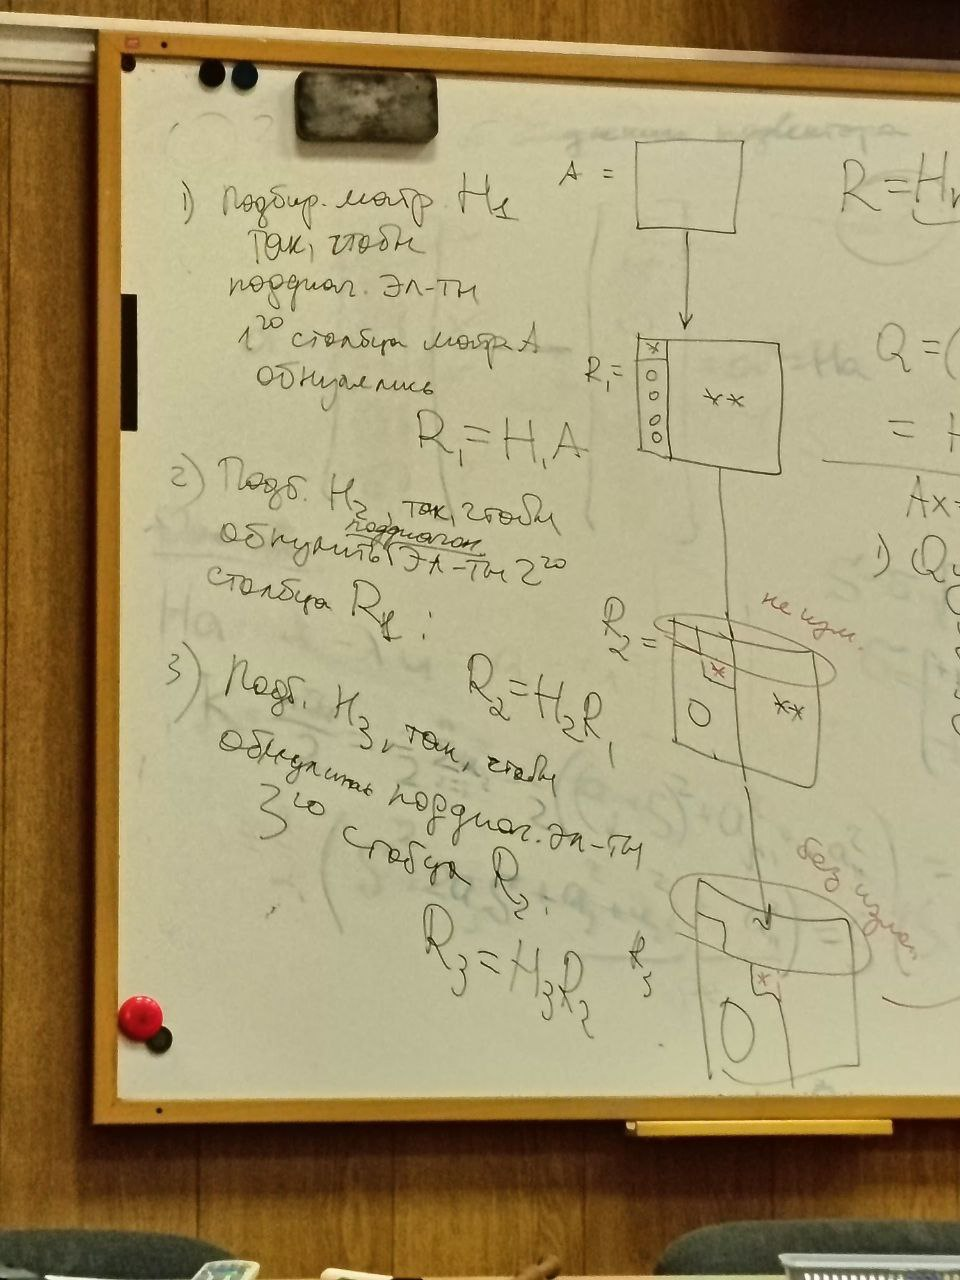
\includegraphics[keepaspectratio]{/home/verz/Документы/Obsidian Vault/Pasted image 20241009193834.png}}\\
  {}\strut \\
  Т.к. {}\\
  {}\strut \\
  Дальнейшее решение - по инструкции\\
  Замечание 1:\\
  Матрицы {} имеют следующую структуру:\\
  {}\strut \\
  {}\strut \\
  Замечание 2:\\
  При выполнении умножения на {} следует оставить без изменения первые
  {} элементы столбца, а нижнюю часть умножить на {} рациональным
  способом
\end{enumerate}

\end{document}
